\newpage
\Question
{ناحیه‌بندی فرکانسی صورت پذیرفته توسط \lr{ITU}}
{
	\lr{ITU} در تنظیم مقررات رادیویی جهانی، جهان را به سه قسمت تقسیم کرده است که هر قسمت تخصیص فرکانسی خاص خود را دارد.
	
	\begin{enumerate}
		\item کشورهای شرق آسیا در جنوب روسیه و ایران
		\item اروپا، آفریقا، روسیه و قسمت غرب خلیج فارس در آسیا
		\item قاره آمریکا
	\end{enumerate}

\begin{figure}[H]
    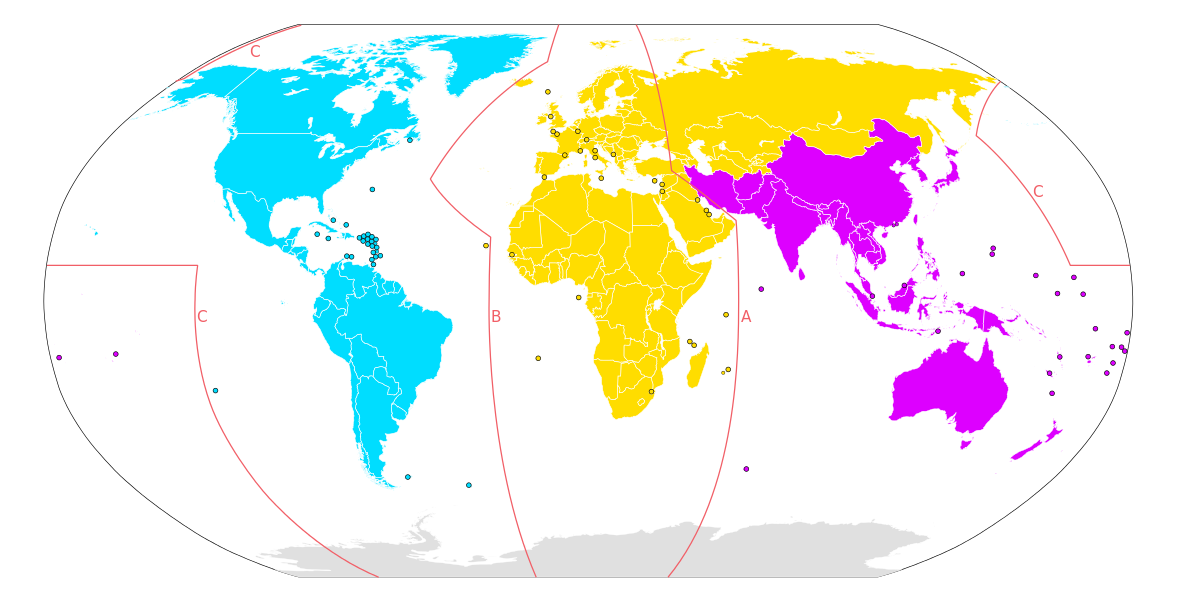
\includegraphics[width=0.85\columnwidth]{Images/ITU_Regions.png}
    \centering
    \caption{قسمت‌های مشخص شده توسط 
    	\lr{ITU}}
\end{figure}
}
